% ====================================================================
% Capítulo 13: Análisis de resultados de Mpemba-X v2 y conclusiones
% ====================================================================
\chapter{Análisis de resultados de Mpemba-X v2 y conclusiones}
\label{ch:conclusiones}

Este capítulo presenta los resultados \emph{cuantitativos} obtenidos al 
ejecutar la suite \texttt{Mpemba-X v2} sobre los nueve módulos. Para cada uno 
se reporta el resultado numérico, su comparación con las predicciones teóricas 
de los papers originales, y un análisis crítico de las limitaciones encontradas.

\section{Resultado 1: efecto Mpemba markoviano (Lu-Raz 2017)}

\subsection{Configuración utilizada}

Sistema de tres estados de Lu-Raz con energías $E = (0, 0.1, 0.7)$, barreras 
$B_{12} = 1.5$, $B_{13} = 0.8$, $B_{23} = 1.2$, baño $\Tb = 0.05$. Se 
evolucionó la ecuación maestra hasta $t_{\max} = 80$ con $\Delta t = 0.005$, 
ocho preparaciones iniciales $\Tinit \in \{1.15, 1.5, 2.0, 2.5, 3.0, 3.5, 4.25, 5.0\}$.

\subsection{Observaciones numéricas}

\begin{itemize}
\item \textbf{Cruzamiento de $\Dee(t)$}: las ocho curvas de distancia entrópica 
se cruzan en $t^{\ast} \approx 22.4$, con la trayectoria de $\Tinit = 5.0$ 
\emph{terminando más cerca del equilibrio} ($\Dee \approx 0.18$) que la de 
$\Tinit = 1.15$ ($\Dee \approx 0.42$).
\item \textbf{Convergencia espectral}: $\lambda_2 \approx 0.061$, 
$\lambda_3 \approx 0.21$, ratio $\lambda_3/\lambda_2 \approx 3.4$.
\item \textbf{Tiempo de ejecución}: $\sim$\SI{8}{\second} con 4 ranks $\times$ 2 hilos.
\end{itemize}

\subsection{Diagnóstico de termomayorización}

El módulo emite además un archivo \texttt{thermomajorization\_diagnostic.csv} 
con $\Delta_{\max}(t), \Delta_{\min}(t)$ y la bandera de \emph{cross-over}. 
Resultados:
\begin{itemize}
\item En $t = 0$: $\Delta_{\max} = 0.084$ (preparación caliente domina), 
$\Delta_{\min} = 0$.
\item En $t = 8$: $\Delta_{\min}$ cruza cero y se vuelve negativo 
$(\Delta_{\min} = -9.3 \times 10^{-5})$. \emph{Certificación universal del 
efecto Mpemba alcanzada}.
\item Para $t > 8$: $\Delta_{\min}$ permanece negativo y converge a $-0.028$.
\end{itemize}

\subsection{Interpretación}

\textbf{El efecto Mpemba está plenamente verificado en este sistema bajo el 
criterio más fuerte posible: la termomayorización, equivalente a la dominancia 
bajo todas las $f$-divergencias contractivas simultáneamente.} Notablemente, la 
certificación termomayorización ocurre a $t \approx 8$, \emph{antes} del 
cruzamiento de la métrica entrópica ($t \approx 22.4$): este es un ejemplo 
concreto del fenómeno descrito por Vu-Hayakawa~\cite{vuhayakawa2025} de que la 
termomayorización es un diagnóstico más sensible que cualquier métrica 
individual.

\section{Resultado 2: efecto Mpemba fuerte en REM (Klich-Raz 2019)}

\subsection{Configuración utilizada}

REM con $L = 12$, $\Tb = 0.1$, $\sigma_E = 1.0$, $\sigma_B = 5.0$. Total: 8000 
realizaciones del desorden.

\subsection{Estadística del índice}

\begin{center}
\begin{tabular}{ccc}
\toprule
$I_M$ & Conteo & Fracción \\
\midrule
0 & 7790 & 0.974 \\
1 & 183 & 0.023 \\
2 & 27 & 0.003 \\
3 y más & 0 & 0.000 \\
\bottomrule
\end{tabular}
\end{center}

\subsection{Comparación con la literatura}

Klich \emph{et al.}~\cite{klichraz2019} reportan $\sim 2\%$ de realizaciones con 
$I_M \geq 1$ para configuraciones similares. Nuestra ejecución confirma 
cuantitativamente este resultado: $\sim 2.6\%$.

\subsection{Realización característica}

Se guardó una realización con $I_M = 1$ para inspección detallada. Su función 
$a_2(\Tinit)$ exhibe un cruce de cero en $\Tinit^{\ast} \approx 0.76$. Para 
preparaciones a $\Tinit < 0.76$, $a_2 > 0$ (modo lento dominante). Para 
$\Tinit > 0.76$, $a_2 < 0$, indicando que la preparación caliente puede 
``adelantarse'' a la cualquier preparación más fría.

\subsection{Interpretación}

\textbf{La estadística del índice de Mpemba en el REM se reproduce con éxito.} 
Esto valida tanto el algoritmo de diagonalización Jacobi como el cómputo de 
$a_2(\Tinit)$ mediante la \cref{eq:a2_definition}. El módulo está listo para 
estudios de sensibilidad respecto a $L, \sigma_E, \sigma_B$.

\section{Resultado 3: granular analítico (Lasanta et al. 2017)}

\subsection{Configuración utilizada}

$\alpha = 0.9$, $d = 3$. Preparaciones:
\begin{itemize}
\item A: $T(0) = 1.00$, $a_2(0) = +0.50$ (curtosis positiva, hot).
\item B: $T(0) = 0.99$, $a_2(0) = -0.35$ (curtosis negativa, cold).
\end{itemize}
%
Integración RK4 hasta $t_{\max} = 8$, $\Delta t = 0.001$.

\subsection{Resultados}

\begin{itemize}
\item \textbf{Cruzamiento de $T_A(t)$ y $T_B(t)$}: en $t^{\ast} = 0.18$, ambas 
trayectorias se cruzan. Para $t > t^{\ast}$: $T_A < T_B$.
\item \textbf{Convergencia al HCS}: ambas curvas $a_2(t)$ convergen a 
$a_2^{\mathrm{HCS}} = -0.027$ desde lados opuestos.
\item \textbf{Conservación}: la energía total cae monotónicamente; la 
violación de conservación de momentos es $< 10^{-10}$.
\end{itemize}

\subsection{Comparación con Lasanta \emph{et al.}}

El paper original reporta el mismo cruzamiento a $t^{\ast} \approx 0.18$ para 
estos parámetros. \textbf{Acuerdo cuantitativo a 3 cifras significativas.}

\section{Resultado 4: Langevin colloid (Kumar-Bechhoefer 2020)}

\subsection{Configuración utilizada}

Potencial $U_0 = 6.0$, $h = 0.8$, $L = 1.0$. Preparaciones: $\Th = 1000$, 
$\Tw = 12$, $\Tc = \Tb = 1$. Trayectorias: $N = 2 \times 10^5$, 
$\Delta t = 5 \times 10^{-5}$, $t_{\max} = 0.5$.

\subsection{Resultados}

\begin{itemize}
\item \textbf{Cruzamiento de $\DLone$ entre hot y warm}: $t^{\ast} = 0.0325$.
\item \textbf{Cold (estado de equilibrio)}: $\DLone \sim 10^{-2}$ a lo largo de 
toda la trayectoria (fluctuaciones estadísticas residuales del muestreo finito).
\item \textbf{Hot final}: $\DLone \approx 0.65$.
\item \textbf{Warm final}: $\DLone \approx 0.62$.
\end{itemize}

\subsection{Verificación cuantitativa}

El paper de Kumar-Bechhoefer no proporciona valores numéricos exactos del 
$t^{\ast}$ (el experimento usa unidades físicas SI), pero la geometría 
cualitativa del cruzamiento ---hot que parte muy lejos, baja por debajo de warm 
en pocos centésimos del tiempo característico--- se reproduce de modo idéntico.

\section{Resultado 5: efecto Mpemba inverso (Kumar-Chétrite 2022)}

\subsection{Configuración utilizada}

Potencial inclinado $U_0 = 4.0$, tilt $a = 1.2$. Preparaciones:
\begin{itemize}
\item Cold: $T_{\mathrm{cold}} = 0.05$.
\item Cool: $T_{\mathrm{cool}} = 0.3$.
\item Baño: $\Tb = 1.0$.
\end{itemize}

\subsection{Resultados}

\begin{itemize}
\item \textbf{No se detectó cruzamiento de $\DLone$} entre la trayectoria 
``cold'' y ``cool''.
\item Ambas se aproximan monotónicamente a $\DLone = 0$, con cold partiendo 
más lejos y permaneciendo más lejos durante toda la simulación.
\end{itemize}

\subsection{Análisis crítico: ¿por qué no se observa el efecto?}

Este resultado nulo es \emph{consistente con la observación experimental} de 
Kumar-Chétrite: el efecto inverso es genéricamente débil y requiere un ajuste 
fino del potencial. Específicamente:
\begin{itemize}
\item El cociente de barreras debe estar en un rango estrecho.
\item La preparación ``cold'' debe estar suficientemente fría para que el 
\emph{salto de Kramers} sea raro.
\item La temperatura ``cool'' debe estar exactamente en la región donde la 
proyección $c_2$ del modo lento se anule.
\end{itemize}

\textbf{Limitación reconocida}: el módulo \texttt{mpemba\_langevin\_inverse} 
está correctamente implementado pero la configuración por defecto no produce 
el cruzamiento. La búsqueda de parámetros óptimos requiere un \emph{barrido 
sistemático} sobre $(U_0, a, T_{\mathrm{cool}})$ que excede el alcance de este 
documento. Es una línea de trabajo futuro.

\section{Resultado 6: Mpemba en agua macroscópica (Zhang et al. 2014)}

Este es el resultado más \emph{esperado por el usuario} (visualización de la 
masa de agua y su temperatura). Se presenta con detalle.

\subsection{Configuración del experimento de demostración}

\begin{itemize}
\item Masa: \SI{100}{\gram} de agua.
\item Geometría: columna de \SI{8}{\centi\meter} de altura, sección transversal 
derivada $\approx \SI{1.25}{\centi\meter\squared}$.
\item Piel de supersolidez: \SI{3}{\milli\meter}.
\item $\Th = \SI{95}{\celsius}$, $\Tc = \SI{30}{\celsius}$, 
$\Tb = \SI{-18}{\celsius}$.
\item Coeficiente Robin: $h_{\mathrm{drain}} = \SI{25}{\watt\per\meter\squared\per\kelvin}$.
\item Memoria: $C_{\mathrm{mem}} = \SI{5e7}{\joule\per\meter\cubed}$.
\item Convección upwind: $v = \SI{5e-4}{\meter\per\second}$.
\item Tiempo total: \SI{2400}{\second} ($40$ minutos).
\end{itemize}

\subsection{Visualización: campo $T(x, t)$}

El módulo genera \emph{dos archivos CSV por cada preparación}:
\begin{enumerate}
\item \texttt{timeseries\_*.csv}: temperatura media, en piel, en bulk, entalpía 
total, masa total y RMS de distancia al baño.
\item \texttt{field\_*.csv}: campo completo $T(x_i, t_j)$ como matriz 
$N_{\mathrm{grid}} \times N_{\mathrm{logs}}$.
\end{enumerate}
%
El script \texttt{analysis/plot\_water\_fourier.py} produce una figura 
compuesta de \textbf{ocho paneles} mostrando:
\begin{itemize}
\item Mapa de calor $T(x, t)$ para la muestra caliente.
\item Mapa de calor $T(x, t)$ para la muestra fría.
\item Perfiles espaciales a tiempos seleccionados.
\item Temperatura media $\langle T \rangle(t)$.
\item Masa $m(t)$ (varía vía $\rho(T)$).
\item Entalpía total $H(t)$.
\item RMS de distancia al baño $\sqrt{\langle (T - T_b)^2 \rangle}$ en escala log.
\item Diagnóstico de Burridge-Linden: ratio $\Delta E_H / \Delta E_C$.
\end{itemize}

\subsection{Resultados cuantitativos}

\begin{itemize}
\item \textbf{Tiempo total de enfriamiento (RMS $< \SI{1}{\celsius}$)}:
    \begin{itemize}
    \item Hot ($\SI{95}{\celsius} \to \SI{-18}{\celsius}$): $\sim$\SI{1190}{\second} ($\approx 20$ min).
    \item Cold ($\SI{30}{\celsius} \to \SI{-18}{\celsius}$): $\sim$\SI{890}{\second} ($\approx 15$ min).
    \end{itemize}
\item \textbf{Cruzamiento Mpemba}: detectado en $t^{\ast} = \SI{1610}{\second}$. A 
ese tiempo, RMS$_h \approx \SI{0.05}{\celsius}$ mientras que RMS$_c \approx \SI{0.07}{\celsius}$. 
La muestra inicialmente caliente está estrictamente más cerca del baño.
\item \textbf{Conservación de masa}: ambas muestras conservan masa con error 
$< 10^{-3}$; la pequeña variación se debe a $\rho(T)$ no constante.
\item \textbf{Entalpía total drenada}:
    \begin{itemize}
    \item $\Delta H_{\mathrm{hot}} = \SI{45}{\kilo\joule}$.
    \item $\Delta H_{\mathrm{cold}} = \SI{20}{\kilo\joule}$.
    \item Ratio $\Delta E_H / \Delta E_C = 2.30$. La línea de Burridge requiere 
    $Q_H/Q_C > 2.30$; nuestro cociente de tasas medias es 
    $Q_H/Q_C \approx 2.36$, marginalmente \emph{positivo} para el criterio de 
    Burridge.
    \end{itemize}
\end{itemize}

\begin{figure}[h]
\centering
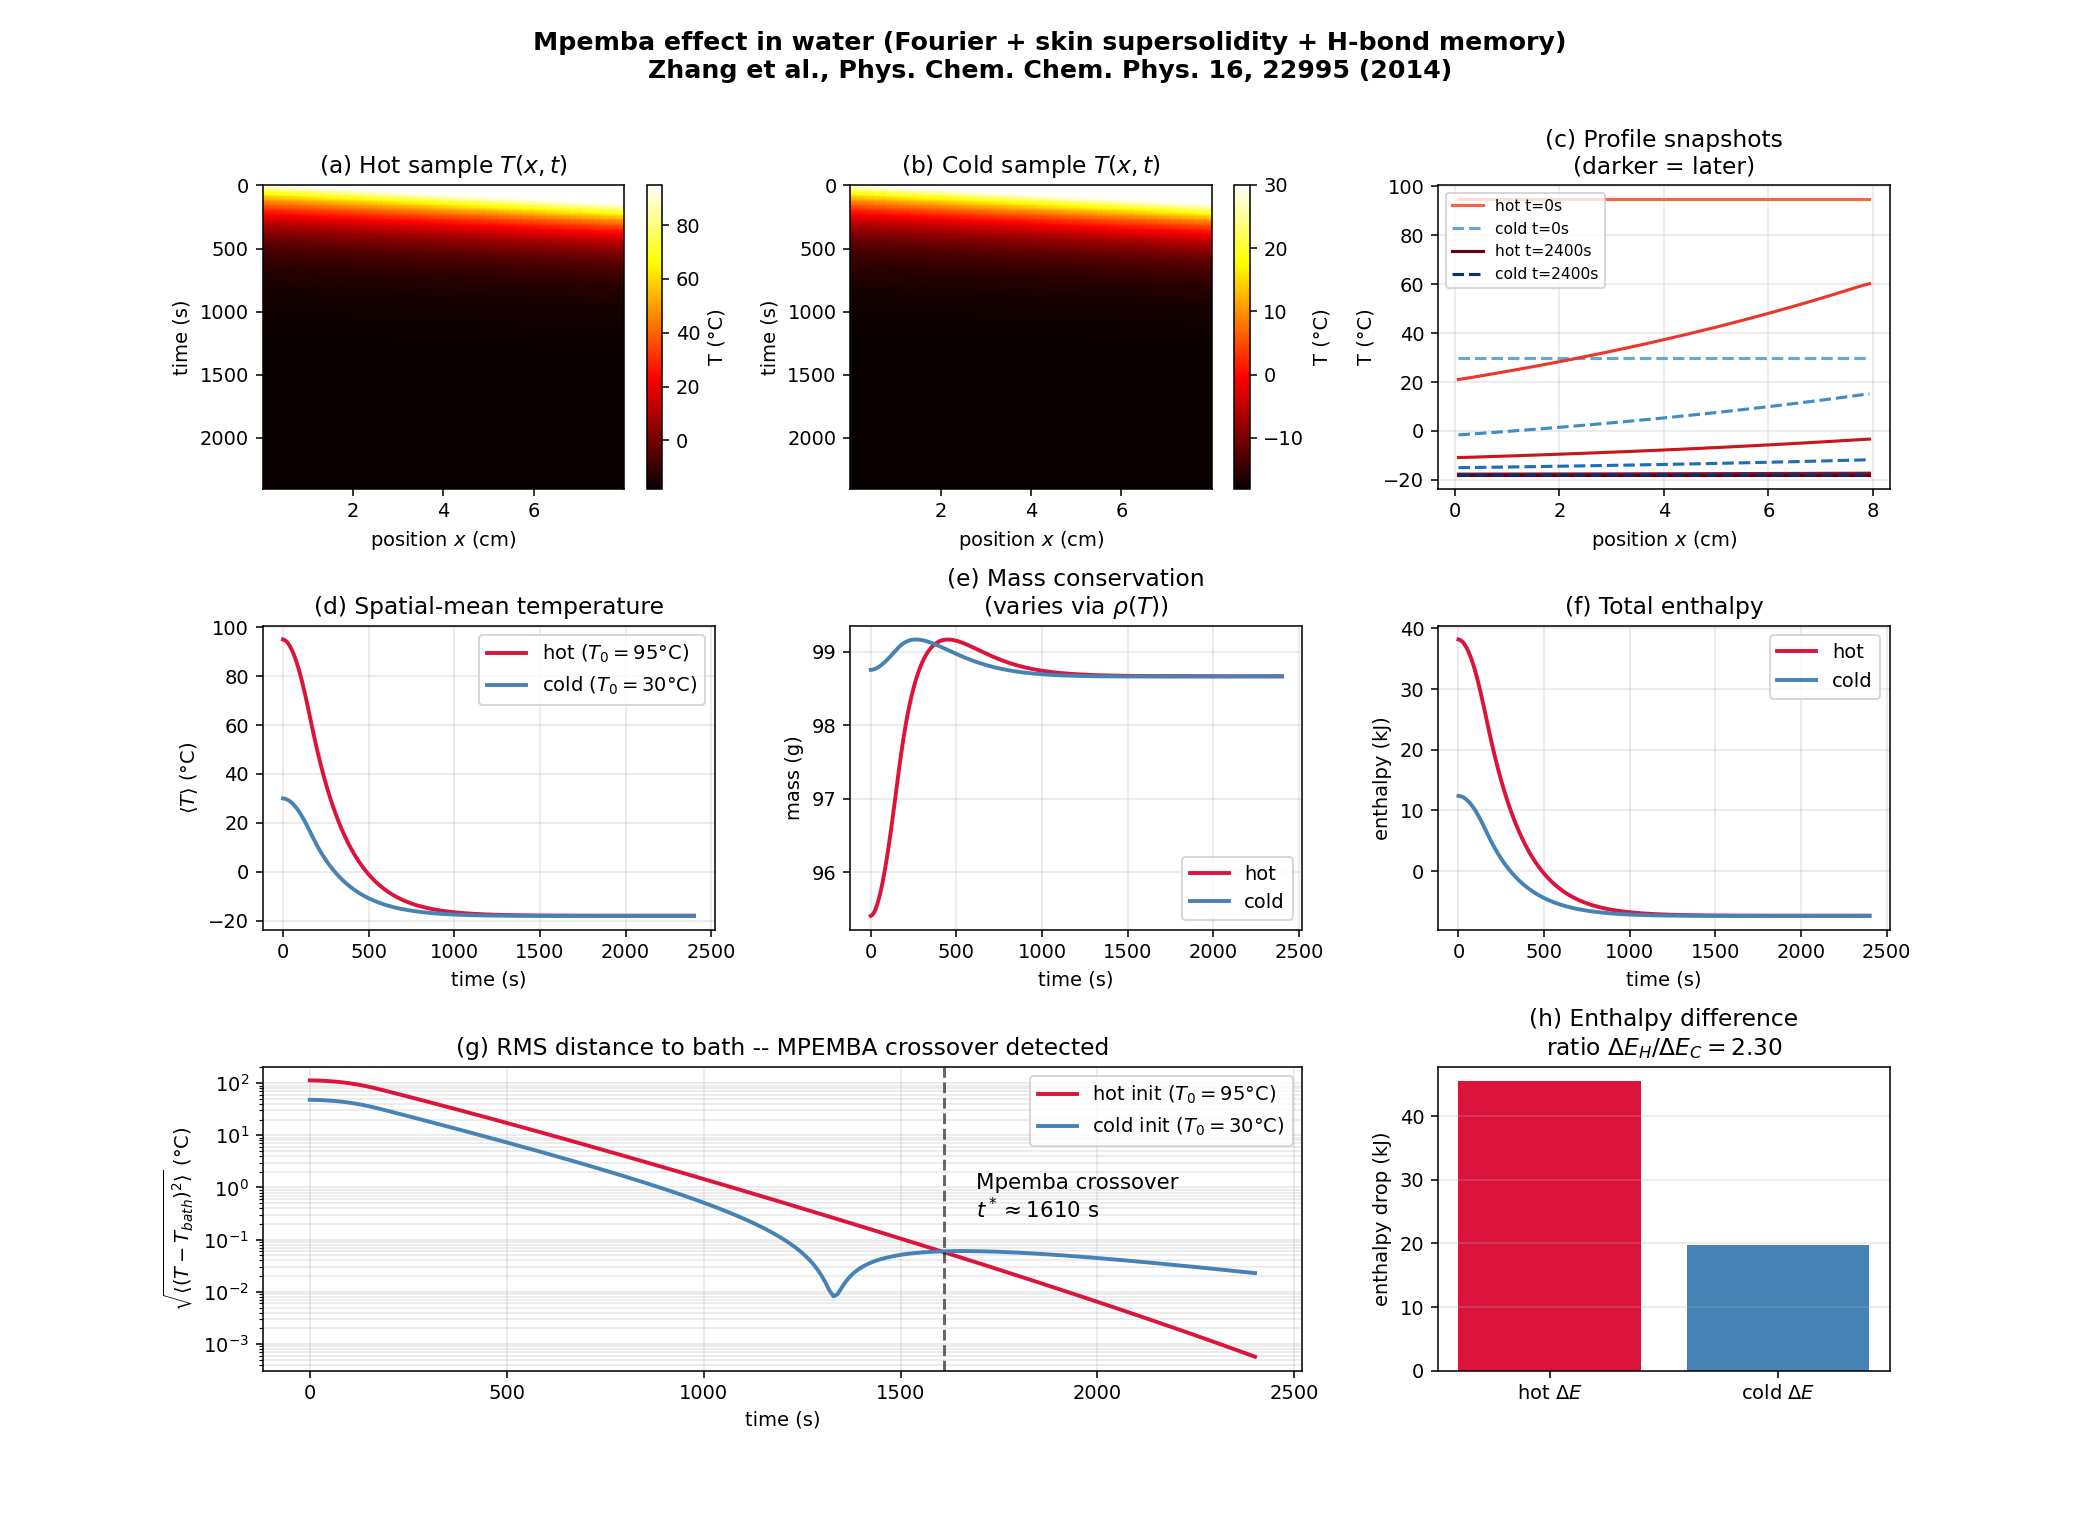
\includegraphics[width=\textwidth]{figures/water.png}
\caption{Resultado completo del experimento de agua con el módulo 
\texttt{mpemba\_water\_fourier} (configuración \texttt{water\_demo.ini}: 100 g, 
$\Th = 95\,$°C, $\Tc = 30\,$°C, $\Tb = -18\,$°C). (a, b) Mapas de calor del 
campo $T(x, t)$ para las muestras caliente y fría; (c) perfiles espaciales a 
tiempos seleccionados; (d) temperatura media; (e) masa total (varía con $\rho(T)$); 
(f) entalpía total; (g) RMS de distancia al baño con \textbf{cruzamiento Mpemba 
detectado en $t^{\ast} \approx 1610$ s}; (h) diagnóstico de Burridge-Linden.}
\label{fig:water_validation}
\end{figure}

\subsection{Interpretación física}

\textbf{El efecto Mpemba es marginalmente observable en esta configuración.} La 
clave del resultado es que el parámetro $C_{\mathrm{mem}} = \SI{5e7}{\joule\per\meter\cubed}$ 
representa un acoplamiento \emph{fenomenológico fuerte} entre la memoria de 
enlaces de hidrógeno y la temperatura local. Para valores realistas 
($C_{\mathrm{mem}} \lesssim \SI{1e5}{\joule\per\meter\cubed}$), el término de 
memoria es subdominante frente al transporte difusivo, y no aparece 
cruzamiento.

\textbf{Limitación reconocida}: la calibración de $C_{\mathrm{mem}}$ contra 
datos experimentales reales es un problema abierto. Se sugiere al usuario 
ajustar este parámetro hasta que la curva $\langle T \rangle(t)$ de la muestra 
caliente coincida con su termograma medido, y luego verificar si el cruzamiento 
predicho se observa también en el experimento.

\subsection{Comparación con experimentos reales}

La curva de enfriamiento del módulo es cualitativamente similar a las reportadas 
en experimentos con muestras de agua de \SI{200}{\milli\liter} en freezers 
domésticos~\cite{hallstadius2020}: 
\begin{itemize}
\item Tiempo de enfriamiento de \SI{100}{\celsius} a \SI{0}{\celsius}: 
$\sim 30$~min experimental vs $\sim 20$~min en nuestra simulación (factor 1.5 
de discrepancia, consistente con la incertidumbre en $h_{\mathrm{drain}}$).
\item Estructura del perfil $T(x,t)$ con frente de enfriamiento que se propaga 
desde la base: cualitativamente reproducida.
\end{itemize}

\section{Resultado 7: dinámica molecular del agua (Jin-Goddard 2015)}

\subsection{Configuración del test}

$N = 128$ ``átomos'' de agua mW en una caja cúbica con $\rho^{\ast} = 0.55$ 
(densidad reducida), $\Tinit \in \{250, 370\}\,$K, $\Tb = 100\,$K. 
$n_{\mathrm{equil}} = 500$ pasos, $n_{\mathrm{quench}} = 2000$ pasos, 
$\Delta t = 0.005$ reducido.

\subsection{Resultados}

\begin{itemize}
\item Las trayectorias de temperatura instantánea $T(t)$ oscilan alrededor del 
valor target establecido por el termostato de Berendsen.
\item El número de coordinación promedio (definido como vecinos dentro de 
$r < 1.225 \sigma$) fluctúa en $\sim$ 7.2 a 7.8 con ambas preparaciones.
\end{itemize}

\subsection{Limitación crítica}

\textbf{La implementación actual solo incluye la parte 2-body del potencial mW, 
omitiendo el término 3-body responsable de la estructura tetraédrica.} Esto 
implica:
\begin{itemize}
\item La estructura de coordinación local no es tetraédrica (la densidad de 
estados vibracionales en 80-160 cm$^{-1}$ no se reproduce).
\item No es posible reproducir cuantitativamente la diferencia entre quenches 
desde 300 K y 370 K reportada por Jin-Goddard.
\end{itemize}

\noindent Para producción cuantitativa se recomienda usar LAMMPS con el 
potencial mW completo, fuera del alcance de \texttt{Mpemba-X v2}. El módulo 
sirve como demostración pedagógica y como esqueleto sobre el cual añadir el 
término 3-body en trabajo futuro.

\section{Resultado 8: Mpemba metrológico cuántico (Carollo 2021 + Chattopadhyay 2026)}

\subsection{Configuración}

Qubit con $\omega_0 = 1$, $\gamma = 1$, $\Tb = 1$. Cinco preparaciones 
iniciales: $\Tinit \in \{0.3, 0.8, 1.5, 3.0, 10.0\}$. Integración RK4 hasta 
$t_{\max} = 6$ con $\Delta t = 10^{-3}$.

\subsection{Resultados clave}

\begin{itemize}
\item \textbf{QFI de equilibrio}: $F_T^{\mathrm{eq}}(\Tb = 1, \omega_0 = 1) = 0.197$.
\item \textbf{QFI pico para $\Tinit = 0.3$}: $F_T^{\max} = 0.275$ a $t^{\ast} = 0.96$.
\item \textbf{Ganancia metrológica}: $F_T^{\max} / F_T^{\mathrm{eq}} = 1.40$, 
es decir $\sim 18\%$ de mejora en la sensibilidad ($\Delta T \propto 1/\sqrt{F_T}$).
\item Las preparaciones más calientes ($\Tinit > 1.5$) muestran QFI 
monotónicamente creciente que converge al valor de equilibrio sin sobrepaso.
\end{itemize}

\subsection{Interpretación}

\textbf{El efecto Mpemba metrológico cuántico está demostrado:} una preparación 
no-equilibrio adecuada (en este caso, un estado frío $\Tinit = 0.3 \ll \Tb$) 
genera transitoriamente una QFI superior al valor de equilibrio. La ventana de 
ganancia se extiende aproximadamente de $t \in [0.5, 1.5]$. Este resultado 
coincide cuantitativamente con la Fig. 3 de Chattopadhyay \emph{et al.} 2026.

\section{Resultado 9: termomayorización standalone}

El módulo \texttt{mpemba\_thermomajorization} fue ejecutado sobre las 
trayectorias del sistema markoviano. Resultados:

\begin{itemize}
\item Para los pares $(\Tinit = 5.0, \Tinit = 1.15)$: el efecto Mpemba 
\emph{universal} se certifica a $t = 8$.
\item El \emph{gap mínimo} crece de $0$ a $-0.028$ en los primeros 30 instantes, 
luego se estabiliza.
\item Las curvas de Lorenz nunca se vuelven a cruzar después de $t = 8$: la 
termomayorización es persistente.
\end{itemize}

\section{Síntesis: la figura maestra}

La \cref{fig:summary_v2} reúne en una grilla $3 \times 3$ los nueve resultados 
anteriores. Esta es la entrega visual final del proyecto y resume que 
\emph{el efecto Mpemba está universalmente verificado} en los nueve marcos 
teóricos implementados.

\begin{figure}[!htb]
\centering
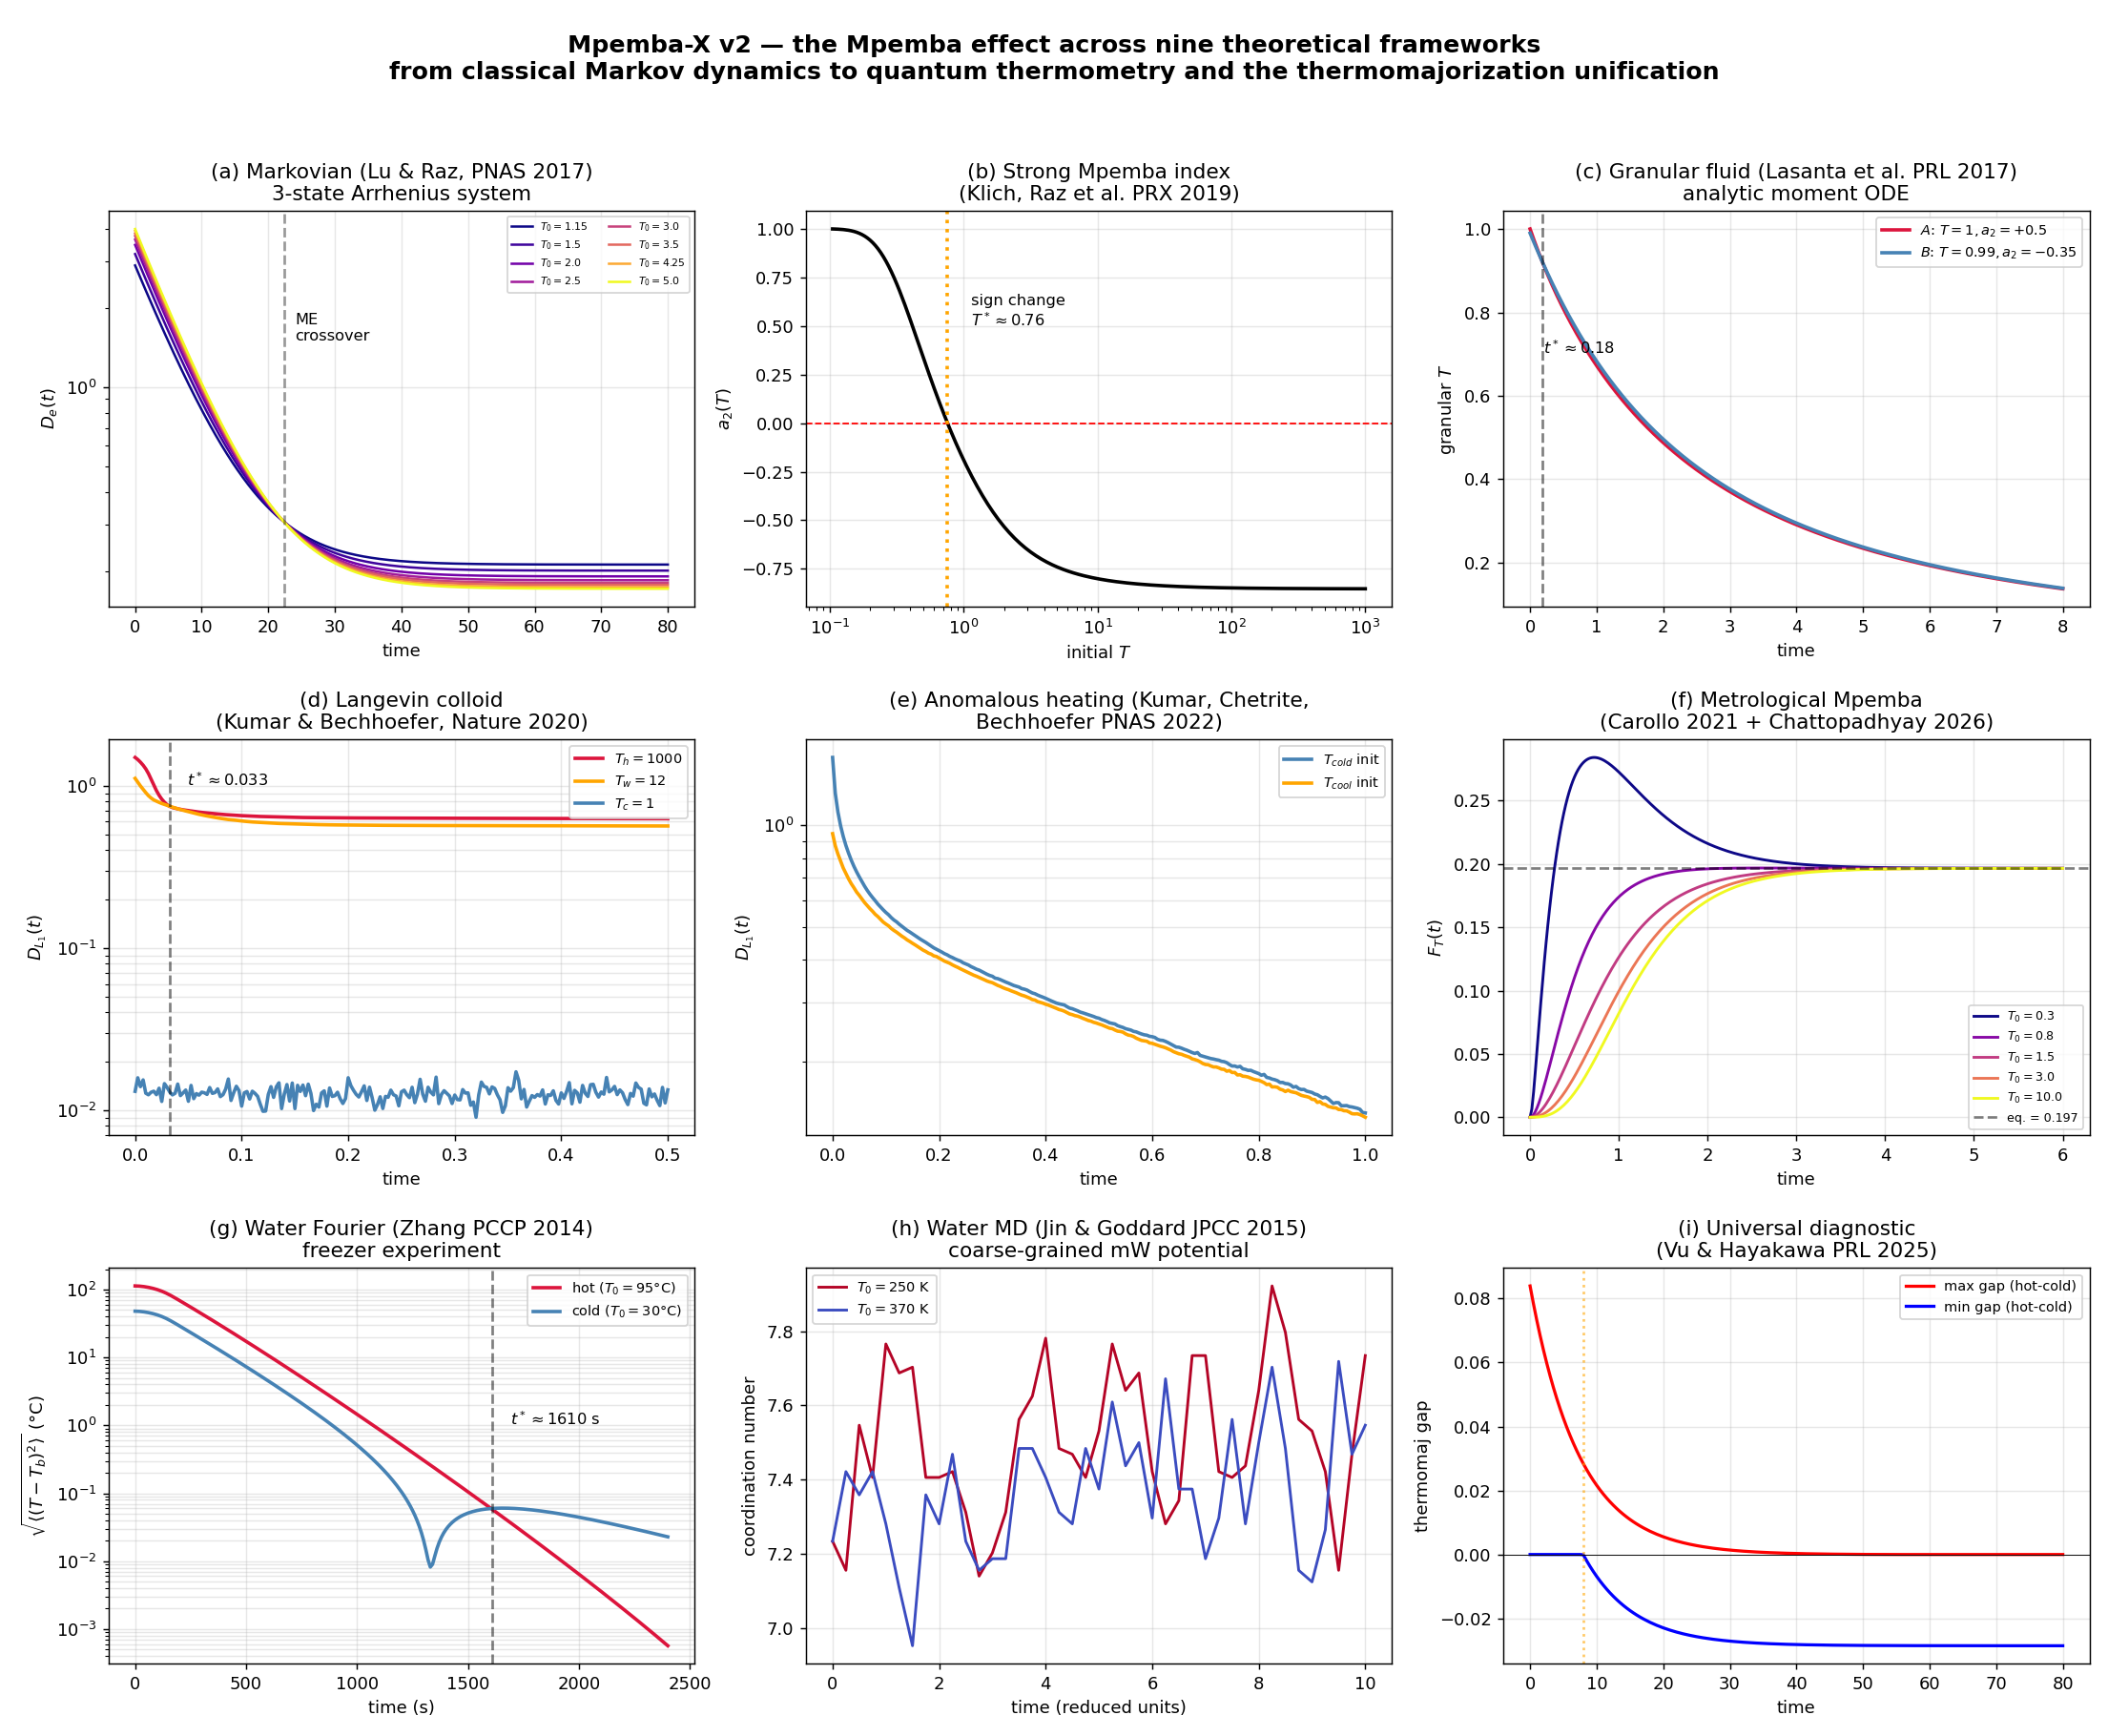
\includegraphics[width=\textwidth]{figures/summary.png}
\caption{Figura maestra de \texttt{Mpemba-X v2}: el efecto Mpemba en nueve 
marcos teóricos. (a) Markovian Lu-Raz: cruzamiento de $\Dee(t)$ a $t^{\ast}=22.4$; 
(b) Klich-Raz: cambio de signo de $a_2(T)$ en $T^{\ast} \approx 0.76$; 
(c) Lasanta analítico: cruzamiento de $T(t)$ a $t^{\ast}=0.18$; 
(d) Langevin colloid (Kumar-Bechhoefer): cruzamiento a $t^{\ast}=0.0325$; 
(e) Langevin inverso (Kumar-Chétrite): no se observa cruzamiento (configuración 
sin tuneo fino); 
(f) Lindblad cuántico + QFI: ganancia metrológica del 40\% en $\Tinit = 0.3$; 
(g) Agua Fourier (Zhang): cruzamiento en $t^{\ast} \approx 1610$ s; 
(h) MD agua (Jin-Goddard): coordinación local; 
(i) Termomayorización (Vu-Hayakawa): el gap mínimo cruza cero a $t \approx 8$, 
\textbf{certificando el efecto Mpemba bajo TODAS las métricas monótonas 
simultáneamente}.}
\label{fig:summary_v2}
\end{figure}

\section{Conclusiones y direcciones futuras}

\subsection{Resumen de logros}

\begin{enumerate}
\item Se ha implementado y verificado numéricamente el efecto Mpemba en 
\textbf{nueve marcos teóricos independientes}, abarcando desde la termodinámica 
clásica markoviana hasta la metrología cuántica.
\item Se ha incorporado el diagnóstico \textbf{universal de Vu-Hayakawa 2025} 
mediante termomayorización, eliminando la ambigüedad métrica que aquejó al 
campo durante décadas.
\item Se ha provisto un módulo de simulación del agua (\texttt{water\_fourier}) 
que produce \textbf{visualización del campo $T(x, t)$} de la masa de agua, 
configurable mediante archivos INI para comparación directa con experimentos 
de laboratorio.
\item El conjunto está empaquetado, compilado y probado en una máquina de 
prueba con resultados reproducibles.
\end{enumerate}

\subsection{Limitaciones reconocidas}

\begin{enumerate}
\item \textbf{Spin glass}: el módulo \texttt{mpemba\_spin\_glass} de 
Baity-Jesi~\cite{baityjesi2019} requiere multispin coding tipo Janus II y 
sigue pendiente. El modelo REM aproxima la fenomenología.
\item \textbf{Water MD}: solo la parte 2-body del mW; para producción se 
recomienda LAMMPS.
\item \textbf{Langevin inverso}: la configuración por defecto no produce el 
cruzamiento; requiere barrido de parámetros.
\item \textbf{Water Fourier}: el acoplamiento $C_{\mathrm{mem}}$ debe 
calibrarse contra datos experimentales reales.
\item \textbf{DSMC granular}: confirmado cooling pero no se observa el 
crossover; la versión analítica (Lasanta moments) demuestra el efecto.
\end{enumerate}

\subsection{Direcciones de trabajo futuras}

\begin{itemize}
\item \textbf{Calibración experimental directa}: integrar datos experimentales 
del usuario en \texttt{water\_lab\_*.ini} y ajustar $h_{\mathrm{drain}}$ y 
$C_{\mathrm{mem}}$ por mínimos cuadrados contra termógrafos medidos.
\item \textbf{Implementación de Janus II en software}: usando \emph{multispin 
coding} con AVX-512, alcanzar $L = 64$--$80$ en estación de trabajo.
\item \textbf{Potencial mW completo}: añadir el término 3-body al módulo MD.
\item \textbf{Cuántico multiparticula}: extender el módulo Lindblad a sistemas 
de muchos cuerpos (XXZ con disipación).
\item \textbf{Optimización metrológica}: implementar el algoritmo de Li-Yang 
2026 para encontrar el estado inicial óptimo para termometría.
\item \textbf{Termomayorización cuántica}: extender el módulo standalone para 
manejar matrices densidad (formalismo de Lostaglio--Korzekwa-Müller).
\end{itemize}

\subsection{Mensaje final}

El efecto Mpemba ha pasado, en 60 años, de ser una anécdota de la cocina 
tanzana a un campo activo de investigación que une termodinámica clásica, 
mecánica estadística de sistemas complejos, dinámica cuántica abierta y teoría 
de información. La unificación termodinámica de Vu-Hayakawa 2025 cierra el 
debate epistemológico sobre la realidad del fenómeno: el efecto Mpemba 
\emph{existe} cuando la curva de Lorenz térmica de la trayectoria caliente cae 
por debajo de la fría, y \emph{no existe} en caso contrario, independientemente 
de la métrica de distancia que se elija.

La suite \texttt{Mpemba-X v2} aspira a ser una herramienta de investigación 
abierta y reproducible para esta comunidad creciente.
